\section{Aufbau und Durchführung}
\label{sec:Durchführung}
\subsection{Aufbau und Durchführung}
Der Aufbau der Apparatur findet sich in Abbildung \ref{fig:aufbau} wieder.
\begin{figure}
    \centering
    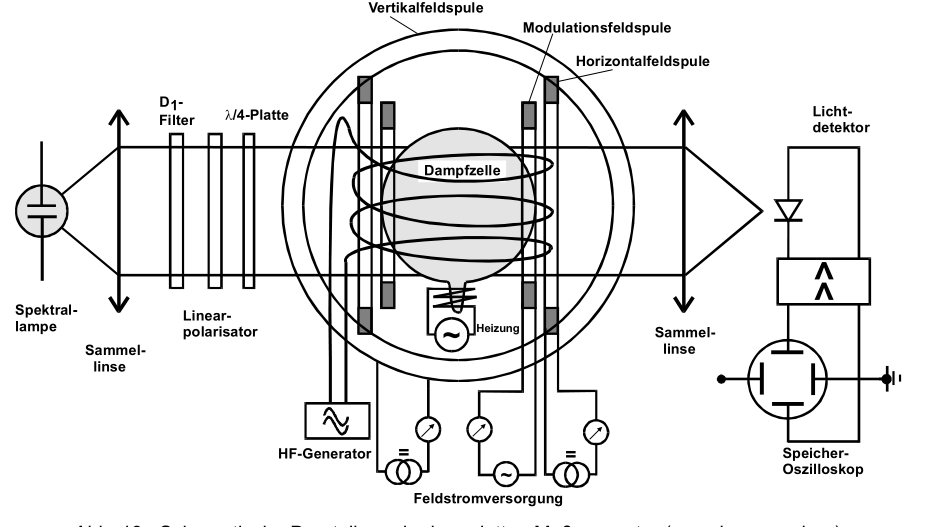
\includegraphics[width=0.5\textwidth]{aufbau.PNG}
    \caption{Der Aufbau der Apparatur.\cite{skript}}
    \label{fig:aufbau}
\end{figure}
Das Licht einer Spektrallampe geht durch einen Interferenzfilter, sodass nur die $D_\mathrm{1}$-Linie
des Rb-Spektrums durchgeht. Dieses unpolarisierte Licht durchläuft eine Zusammensetzung aus Polarisationsfilter
und $\frac{\lambda}{4}$-Platte und wird dadurch zirkular polarisiert.
Eine beheizte Dampfzelle gefüllt mit Rb-Dampf und umhüllt von drei Helmholtz-Spulen, wird vom Licht bestrahlt.
Zwei der Helmholtz-Spulen erzeugen ein horizontales bzw. vertikales Magnetfeld die Dritte, eine Sweep-Spule,
dient zum Regulieren des Magnetfeldes. Ein Si-Photoelment detektiert das durchtretende Licht und wird als Signal
am Oszilloskop ausgegeben.
Die Apparatur ist, zur Minimierung der Einflüsse, in horizontaler Richtung des Erdmagnetfeldes ausgerichtet.
Die Einflüsse lassen sich später in der Auswertung einbinden.
Die Vertikalkomponente des Erdmagnetfeldes wird durch die Vertikalfeldspule ausgeglichen.

Gemessen wird der Strom bei dem Resonanzen auftreten für Frequenzen zwischen $100\si{\kilo\hertz}$ und $1\si{\mega\hertz}$
des Hochfrequenzfeldes.
